\chapter{p3 = 34 (32 graphs)}
\newpage\begin{figure}
  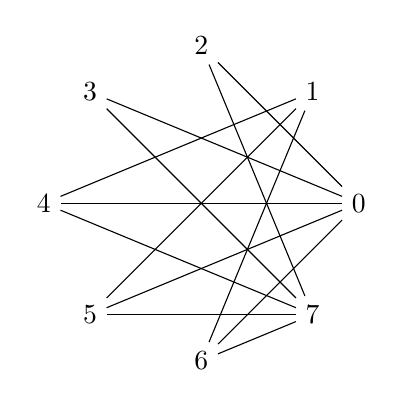
\begin{tikzpicture}
      \draw
        (0.0:2) node (0){0}
        (45.0:2) node (1){1}
        (90.0:2) node (2){2}
        (135.0:2) node (3){3}
        (180.0:2) node (4){4}
        (225.0:2) node (5){5}
        (270.0:2) node (6){6}
        (315.0:2) node (7){7};
      \begin{scope}[-]
        \draw (0) to (2);
        \draw (0) to (3);
        \draw (0) to (4);
        \draw (0) to (5);
        \draw (0) to (6);
        \draw (1) to (4);
        \draw (1) to (5);
        \draw (1) to (6);
        \draw (2) to (7);
        \draw (3) to (7);
        \draw (4) to (7);
        \draw (5) to (7);
        \draw (6) to (7);
      \end{scope}
    \end{tikzpicture}
\end{figure}
\begin{itemize}
\item signature: 0111110001110000010001001011
\item g: Graph with 8 nodes and 13 edges
\item order: 8
\item size: 13
\item max degree: 5
\item degrees: 2,2,3,3,3,3,5,5
\item is tree: 0
\item is bipartite: 1
\item has bridge: 0
\item is chordal: 0
\item is complete: 0
\item min cycle basis weight: 24
\item min cycle basis size: 6
\item diameter: 3
\item radius: 2
\item is eulerian: 0
\item is planar: 0
\item number of faces: 7
\item is regular: 0
\item p3: 34
\item p4: 12
\item property hash: 4c7ab7864c88c491ad7f9527763f1beca29b0f6221ef4cefebac5bfd303aa112
\end{itemize}
\newpage
\begin{figure}
  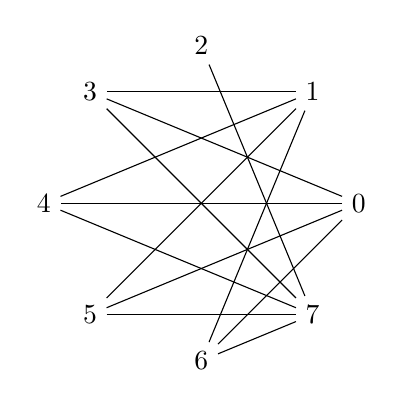
\begin{tikzpicture}
      \draw
        (0.0:2) node (0){0}
        (45.0:2) node (1){1}
        (90.0:2) node (2){2}
        (135.0:2) node (3){3}
        (180.0:2) node (4){4}
        (225.0:2) node (5){5}
        (270.0:2) node (6){6}
        (315.0:2) node (7){7};
      \begin{scope}[-]
        \draw (0) to (3);
        \draw (0) to (4);
        \draw (0) to (5);
        \draw (0) to (6);
        \draw (1) to (3);
        \draw (1) to (4);
        \draw (1) to (5);
        \draw (1) to (6);
        \draw (2) to (7);
        \draw (3) to (7);
        \draw (4) to (7);
        \draw (5) to (7);
        \draw (6) to (7);
      \end{scope}
    \end{tikzpicture}
\end{figure}
\begin{itemize}
\item signature: 0011110011110000010001001011
\item g: Graph with 8 nodes and 13 edges
\item order: 8
\item size: 13
\item max degree: 5
\item degrees: 1,3,3,3,3,4,4,5
\item is tree: 0
\item is bipartite: 1
\item has bridge: 1
\item is chordal: 0
\item is complete: 0
\item min cycle basis weight: 24
\item min cycle basis size: 6
\item diameter: 3
\item radius: 2
\item is eulerian: 0
\item is planar: 0
\item number of faces: 7
\item is regular: 0
\item p3: 34
\item p4: 8
\item property hash: af6b1ed3da94338b68ddf48d69d3bb0b0d5c891b319db757bc33d852b39c194c
\end{itemize}
\newpage
\begin{figure}
  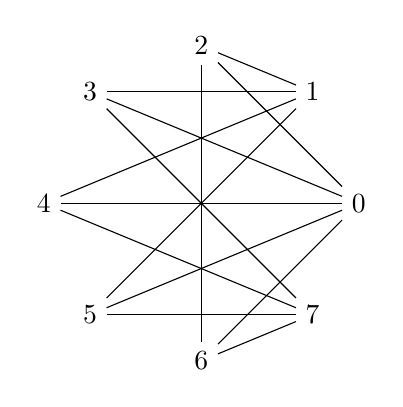
\begin{tikzpicture}
      \draw
        (0.0:2) node (0){0}
        (45.0:2) node (1){1}
        (90.0:2) node (2){2}
        (135.0:2) node (3){3}
        (180.0:2) node (4){4}
        (225.0:2) node (5){5}
        (270.0:2) node (6){6}
        (315.0:2) node (7){7};
      \begin{scope}[-]
        \draw (0) to (2);
        \draw (0) to (3);
        \draw (0) to (4);
        \draw (0) to (5);
        \draw (0) to (6);
        \draw (1) to (2);
        \draw (1) to (3);
        \draw (1) to (4);
        \draw (1) to (5);
        \draw (2) to (6);
        \draw (3) to (7);
        \draw (4) to (7);
        \draw (5) to (7);
        \draw (6) to (7);
      \end{scope}
    \end{tikzpicture}
\end{figure}
\begin{itemize}
\item signature: 0111110111100000100001001011
\item g: Graph with 8 nodes and 14 edges
\item order: 8
\item size: 14
\item max degree: 5
\item degrees: 3,3,3,3,3,4,4,5
\item is tree: 0
\item is bipartite: 0
\item has bridge: 0
\item is chordal: 0
\item is complete: 0
\item min cycle basis weight: 27
\item min cycle basis size: 7
\item diameter: 2
\item radius: 2
\item is eulerian: 0
\item is planar: 0
\item number of faces: 8
\item is regular: 0
\item p3: 34
\item p4: 19
\item property hash: 160cde970dc55f8cb225d520ee17d7e9fb00f9cc2158b1bbbaed02728f898993
\end{itemize}
\newpage
\begin{figure}
  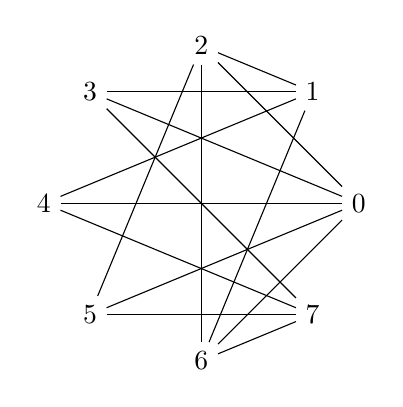
\begin{tikzpicture}
      \draw
        (0.0:2) node (0){0}
        (45.0:2) node (1){1}
        (90.0:2) node (2){2}
        (135.0:2) node (3){3}
        (180.0:2) node (4){4}
        (225.0:2) node (5){5}
        (270.0:2) node (6){6}
        (315.0:2) node (7){7};
      \begin{scope}[-]
        \draw (0) to (2);
        \draw (0) to (3);
        \draw (0) to (4);
        \draw (0) to (5);
        \draw (0) to (6);
        \draw (1) to (2);
        \draw (1) to (3);
        \draw (1) to (4);
        \draw (1) to (6);
        \draw (2) to (5);
        \draw (2) to (6);
        \draw (3) to (7);
        \draw (4) to (7);
        \draw (5) to (7);
        \draw (6) to (7);
      \end{scope}
    \end{tikzpicture}
\end{figure}
\begin{itemize}
\item signature: 0111110111010001100001001011
\item g: Graph with 8 nodes and 15 edges
\item order: 8
\item size: 15
\item max degree: 5
\item degrees: 3,3,3,4,4,4,4,5
\item is tree: 0
\item is bipartite: 0
\item has bridge: 0
\item is chordal: 0
\item is complete: 0
\item min cycle basis weight: 29
\item min cycle basis size: 8
\item diameter: 2
\item radius: 2
\item is eulerian: 0
\item is planar: 0
\item number of faces: 9
\item is regular: 0
\item p3: 34
\item p4: 17
\item property hash: 140980b59327089af18a171f93bd9ab02f3128b6b581e113bc34431148ee9e4e
\end{itemize}
\newpage
\begin{figure}
  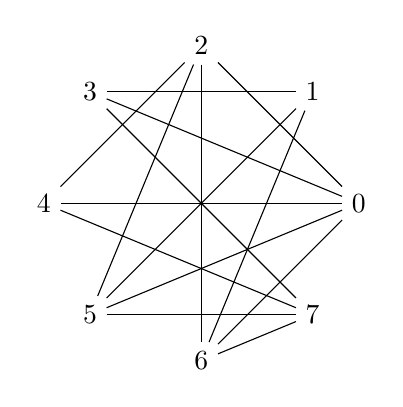
\begin{tikzpicture}
      \draw
        (0.0:2) node (0){0}
        (45.0:2) node (1){1}
        (90.0:2) node (2){2}
        (135.0:2) node (3){3}
        (180.0:2) node (4){4}
        (225.0:2) node (5){5}
        (270.0:2) node (6){6}
        (315.0:2) node (7){7};
      \begin{scope}[-]
        \draw (0) to (2);
        \draw (0) to (3);
        \draw (0) to (4);
        \draw (0) to (5);
        \draw (0) to (6);
        \draw (1) to (3);
        \draw (1) to (5);
        \draw (1) to (6);
        \draw (2) to (4);
        \draw (2) to (5);
        \draw (2) to (6);
        \draw (3) to (7);
        \draw (4) to (7);
        \draw (5) to (7);
        \draw (6) to (7);
      \end{scope}
    \end{tikzpicture}
\end{figure}
\begin{itemize}
\item signature: 0111110010110011100001001011
\item g: Graph with 8 nodes and 15 edges
\item order: 8
\item size: 15
\item max degree: 5
\item degrees: 3,3,3,4,4,4,4,5
\item is tree: 0
\item is bipartite: 0
\item has bridge: 0
\item is chordal: 0
\item is complete: 0
\item min cycle basis weight: 29
\item min cycle basis size: 8
\item diameter: 3
\item radius: 2
\item is eulerian: 0
\item is planar: 0
\item number of faces: 9
\item is regular: 0
\item p3: 34
\item p4: 15
\item property hash: 28c04e89bed59a1efcf690ed2bde69b9120ccd6b1df3775f7d8f898ced79acd5
\end{itemize}
\newpage
\begin{figure}
  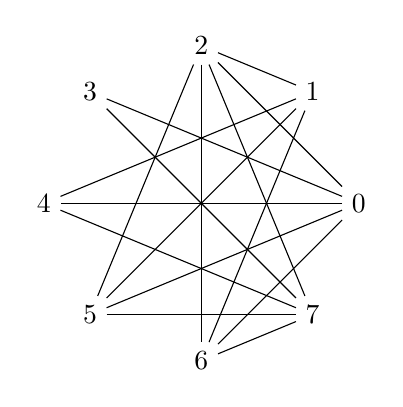
\begin{tikzpicture}
      \draw
        (0.0:2) node (0){0}
        (45.0:2) node (1){1}
        (90.0:2) node (2){2}
        (135.0:2) node (3){3}
        (180.0:2) node (4){4}
        (225.0:2) node (5){5}
        (270.0:2) node (6){6}
        (315.0:2) node (7){7};
      \begin{scope}[-]
        \draw (0) to (2);
        \draw (0) to (3);
        \draw (0) to (4);
        \draw (0) to (5);
        \draw (0) to (6);
        \draw (1) to (2);
        \draw (1) to (4);
        \draw (1) to (5);
        \draw (1) to (6);
        \draw (2) to (5);
        \draw (2) to (6);
        \draw (2) to (7);
        \draw (3) to (7);
        \draw (4) to (7);
        \draw (5) to (7);
        \draw (6) to (7);
      \end{scope}
    \end{tikzpicture}
\end{figure}
\begin{itemize}
\item signature: 0111110101110001110001001011
\item g: Graph with 8 nodes and 16 edges
\item order: 8
\item size: 16
\item max degree: 5
\item degrees: 2,3,4,4,4,5,5,5
\item is tree: 0
\item is bipartite: 0
\item has bridge: 0
\item is chordal: 0
\item is complete: 0
\item min cycle basis weight: 30
\item min cycle basis size: 9
\item diameter: 3
\item radius: 2
\item is eulerian: 0
\item is planar: 0
\item number of faces: 10
\item is regular: 0
\item p3: 34
\item p4: None
\item property hash: 24b45ed1d67004eac51d45097322baf7f126c82da5f7f6b93cc8f4cd15cb9fd4
\end{itemize}
\newpage
\begin{figure}
  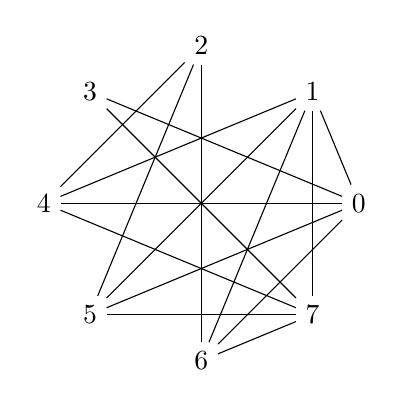
\begin{tikzpicture}
      \draw
        (0.0:2) node (0){0}
        (45.0:2) node (1){1}
        (90.0:2) node (2){2}
        (135.0:2) node (3){3}
        (180.0:2) node (4){4}
        (225.0:2) node (5){5}
        (270.0:2) node (6){6}
        (315.0:2) node (7){7};
      \begin{scope}[-]
        \draw (0) to (1);
        \draw (0) to (3);
        \draw (0) to (4);
        \draw (0) to (5);
        \draw (0) to (6);
        \draw (1) to (4);
        \draw (1) to (5);
        \draw (1) to (6);
        \draw (1) to (7);
        \draw (2) to (4);
        \draw (2) to (5);
        \draw (2) to (6);
        \draw (3) to (7);
        \draw (4) to (7);
        \draw (5) to (7);
        \draw (6) to (7);
      \end{scope}
    \end{tikzpicture}
\end{figure}
\begin{itemize}
\item signature: 1011110001111011100001001011
\item g: Graph with 8 nodes and 16 edges
\item order: 8
\item size: 16
\item max degree: 5
\item degrees: 2,3,4,4,4,5,5,5
\item is tree: 0
\item is bipartite: 0
\item has bridge: 0
\item is chordal: 0
\item is complete: 0
\item min cycle basis weight: 30
\item min cycle basis size: 9
\item diameter: 3
\item radius: 2
\item is eulerian: 0
\item is planar: 0
\item number of faces: 10
\item is regular: 0
\item p3: 34
\item p4: None
\item property hash: 24b45ed1d67004eac51d45097322baf7f126c82da5f7f6b93cc8f4cd15cb9fd4
\end{itemize}
\newpage
\begin{figure}
  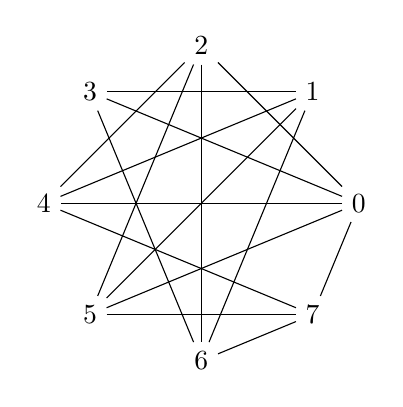
\begin{tikzpicture}
      \draw
        (0.0:2) node (0){0}
        (45.0:2) node (1){1}
        (90.0:2) node (2){2}
        (135.0:2) node (3){3}
        (180.0:2) node (4){4}
        (225.0:2) node (5){5}
        (270.0:2) node (6){6}
        (315.0:2) node (7){7};
      \begin{scope}[-]
        \draw (0) to (2);
        \draw (0) to (3);
        \draw (0) to (4);
        \draw (0) to (5);
        \draw (0) to (7);
        \draw (1) to (3);
        \draw (1) to (4);
        \draw (1) to (5);
        \draw (1) to (6);
        \draw (2) to (4);
        \draw (2) to (5);
        \draw (2) to (6);
        \draw (3) to (6);
        \draw (4) to (7);
        \draw (5) to (7);
        \draw (6) to (7);
      \end{scope}
    \end{tikzpicture}
\end{figure}
\begin{itemize}
\item signature: 0111101011110011100010001011
\item g: Graph with 8 nodes and 16 edges
\item order: 8
\item size: 16
\item max degree: 5
\item degrees: 3,4,4,4,4,4,4,5
\item is tree: 0
\item is bipartite: 0
\item has bridge: 0
\item is chordal: 0
\item is complete: 0
\item min cycle basis weight: 31
\item min cycle basis size: 9
\item diameter: 2
\item radius: 2
\item is eulerian: 0
\item is planar: 0
\item number of faces: 10
\item is regular: 0
\item p3: 34
\item p4: 16
\item property hash: 882257e5b1842d574e5bfb2f5b47da2b0ae77bdbcf85df6de28d78f1f3eb82cf
\end{itemize}
\newpage
\begin{figure}
  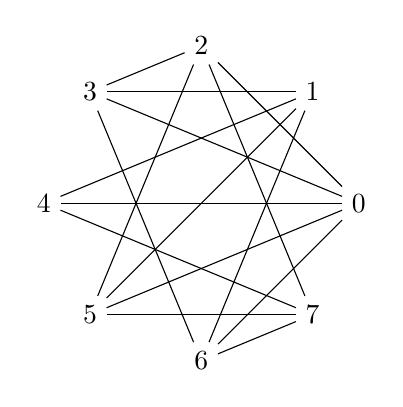
\begin{tikzpicture}
      \draw
        (0.0:2) node (0){0}
        (45.0:2) node (1){1}
        (90.0:2) node (2){2}
        (135.0:2) node (3){3}
        (180.0:2) node (4){4}
        (225.0:2) node (5){5}
        (270.0:2) node (6){6}
        (315.0:2) node (7){7};
      \begin{scope}[-]
        \draw (0) to (2);
        \draw (0) to (3);
        \draw (0) to (4);
        \draw (0) to (5);
        \draw (0) to (6);
        \draw (1) to (3);
        \draw (1) to (4);
        \draw (1) to (5);
        \draw (1) to (6);
        \draw (2) to (3);
        \draw (2) to (5);
        \draw (2) to (7);
        \draw (3) to (6);
        \draw (4) to (7);
        \draw (5) to (7);
        \draw (6) to (7);
      \end{scope}
    \end{tikzpicture}
\end{figure}
\begin{itemize}
\item signature: 0111110011110101010010001011
\item g: Graph with 8 nodes and 16 edges
\item order: 8
\item size: 16
\item max degree: 5
\item degrees: 3,4,4,4,4,4,4,5
\item is tree: 0
\item is bipartite: 0
\item has bridge: 0
\item is chordal: 0
\item is complete: 0
\item min cycle basis weight: 31
\item min cycle basis size: 9
\item diameter: 2
\item radius: 2
\item is eulerian: 0
\item is planar: 0
\item number of faces: 10
\item is regular: 0
\item p3: 34
\item p4: 16
\item property hash: 882257e5b1842d574e5bfb2f5b47da2b0ae77bdbcf85df6de28d78f1f3eb82cf
\end{itemize}
\newpage
\begin{figure}
  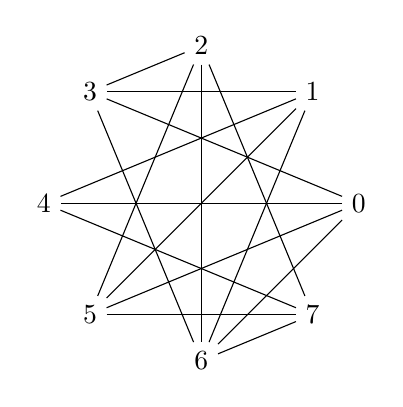
\begin{tikzpicture}
      \draw
        (0.0:2) node (0){0}
        (45.0:2) node (1){1}
        (90.0:2) node (2){2}
        (135.0:2) node (3){3}
        (180.0:2) node (4){4}
        (225.0:2) node (5){5}
        (270.0:2) node (6){6}
        (315.0:2) node (7){7};
      \begin{scope}[-]
        \draw (0) to (3);
        \draw (0) to (4);
        \draw (0) to (5);
        \draw (0) to (6);
        \draw (1) to (3);
        \draw (1) to (4);
        \draw (1) to (5);
        \draw (1) to (6);
        \draw (2) to (3);
        \draw (2) to (5);
        \draw (2) to (6);
        \draw (2) to (7);
        \draw (3) to (6);
        \draw (4) to (7);
        \draw (5) to (7);
        \draw (6) to (7);
      \end{scope}
    \end{tikzpicture}
\end{figure}
\begin{itemize}
\item signature: 0011110011110101110010001011
\item g: Graph with 8 nodes and 16 edges
\item order: 8
\item size: 16
\item max degree: 5
\item degrees: 3,4,4,4,4,4,4,5
\item is tree: 0
\item is bipartite: 0
\item has bridge: 0
\item is chordal: 0
\item is complete: 0
\item min cycle basis weight: 31
\item min cycle basis size: 9
\item diameter: 2
\item radius: 2
\item is eulerian: 0
\item is planar: 0
\item number of faces: 10
\item is regular: 0
\item p3: 34
\item p4: 17
\item property hash: 591aa2bfc2443684a6efb6e3f4d22078d4e62c9f42ed154b23f62689e272d6b7
\end{itemize}
\newpage
\begin{figure}
  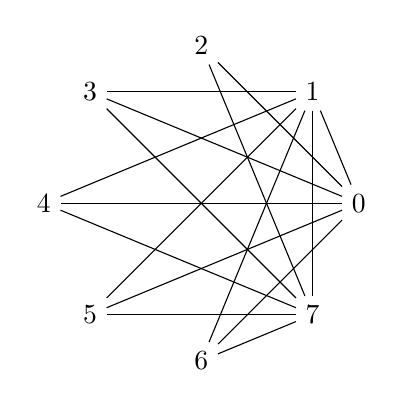
\begin{tikzpicture}
      \draw
        (0.0:2) node (0){0}
        (45.0:2) node (1){1}
        (90.0:2) node (2){2}
        (135.0:2) node (3){3}
        (180.0:2) node (4){4}
        (225.0:2) node (5){5}
        (270.0:2) node (6){6}
        (315.0:2) node (7){7};
      \begin{scope}[-]
        \draw (0) to (1);
        \draw (0) to (2);
        \draw (0) to (3);
        \draw (0) to (4);
        \draw (0) to (5);
        \draw (0) to (6);
        \draw (1) to (3);
        \draw (1) to (4);
        \draw (1) to (5);
        \draw (1) to (6);
        \draw (1) to (7);
        \draw (2) to (7);
        \draw (3) to (7);
        \draw (4) to (7);
        \draw (5) to (7);
        \draw (6) to (7);
      \end{scope}
    \end{tikzpicture}
\end{figure}
\begin{itemize}
\item signature: 1111110011111000010001001011
\item g: Graph with 8 nodes and 16 edges
\item order: 8
\item size: 16
\item max degree: 6
\item degrees: 2,3,3,3,3,6,6,6
\item is tree: 0
\item is bipartite: 0
\item has bridge: 0
\item is chordal: 0
\item is complete: 0
\item min cycle basis weight: 28
\item min cycle basis size: 9
\item diameter: 2
\item radius: 2
\item is eulerian: 0
\item is planar: 0
\item number of faces: 10
\item is regular: 0
\item p3: 34
\item p4: None
\item property hash: 91ae63756a09379d7dceb54979e7aab3f7e3e3b2ca2ef6824f3d0f3bce5b4c5e
\end{itemize}
\newpage
\begin{figure}
  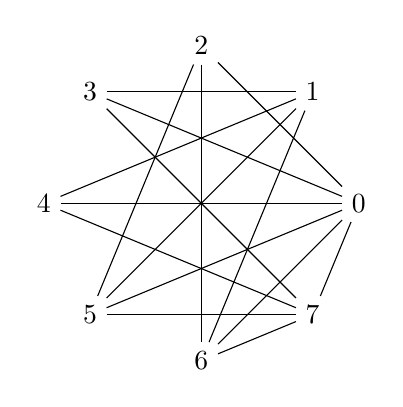
\begin{tikzpicture}
      \draw
        (0.0:2) node (0){0}
        (45.0:2) node (1){1}
        (90.0:2) node (2){2}
        (135.0:2) node (3){3}
        (180.0:2) node (4){4}
        (225.0:2) node (5){5}
        (270.0:2) node (6){6}
        (315.0:2) node (7){7};
      \begin{scope}[-]
        \draw (0) to (2);
        \draw (0) to (3);
        \draw (0) to (4);
        \draw (0) to (5);
        \draw (0) to (6);
        \draw (0) to (7);
        \draw (1) to (3);
        \draw (1) to (4);
        \draw (1) to (5);
        \draw (1) to (6);
        \draw (2) to (5);
        \draw (2) to (6);
        \draw (3) to (7);
        \draw (4) to (7);
        \draw (5) to (7);
        \draw (6) to (7);
      \end{scope}
    \end{tikzpicture}
\end{figure}
\begin{itemize}
\item signature: 0111111011110001100001001011
\item g: Graph with 8 nodes and 16 edges
\item order: 8
\item size: 16
\item max degree: 6
\item degrees: 3,3,3,4,4,4,5,6
\item is tree: 0
\item is bipartite: 0
\item has bridge: 0
\item is chordal: 0
\item is complete: 0
\item min cycle basis weight: 30
\item min cycle basis size: 9
\item diameter: 2
\item radius: 2
\item is eulerian: 0
\item is planar: 0
\item number of faces: 10
\item is regular: 0
\item p3: 34
\item p4: None
\item property hash: f75e701bb1e3546479181ccdf40a776d7635a33f79481df199646a1d24eda258
\end{itemize}
\newpage
\begin{figure}
  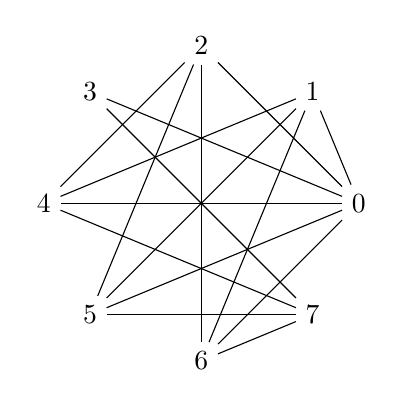
\begin{tikzpicture}
      \draw
        (0.0:2) node (0){0}
        (45.0:2) node (1){1}
        (90.0:2) node (2){2}
        (135.0:2) node (3){3}
        (180.0:2) node (4){4}
        (225.0:2) node (5){5}
        (270.0:2) node (6){6}
        (315.0:2) node (7){7};
      \begin{scope}[-]
        \draw (0) to (1);
        \draw (0) to (2);
        \draw (0) to (3);
        \draw (0) to (4);
        \draw (0) to (5);
        \draw (0) to (6);
        \draw (1) to (4);
        \draw (1) to (5);
        \draw (1) to (6);
        \draw (2) to (4);
        \draw (2) to (5);
        \draw (2) to (6);
        \draw (3) to (7);
        \draw (4) to (7);
        \draw (5) to (7);
        \draw (6) to (7);
      \end{scope}
    \end{tikzpicture}
\end{figure}
\begin{itemize}
\item signature: 1111110001110011100001001011
\item g: Graph with 8 nodes and 16 edges
\item order: 8
\item size: 16
\item max degree: 6
\item degrees: 2,4,4,4,4,4,4,6
\item is tree: 0
\item is bipartite: 0
\item has bridge: 0
\item is chordal: 0
\item is complete: 0
\item min cycle basis weight: 30
\item min cycle basis size: 9
\item diameter: 2
\item radius: 2
\item is eulerian: 1
\item is planar: 0
\item number of faces: 10
\item is regular: 0
\item p3: 34
\item p4: None
\item property hash: 7aa6358cddb9b7b4f208622c3fe5390a6e717c0d8d185073f943f41d3f4b3ff4
\end{itemize}
\newpage
\begin{figure}
  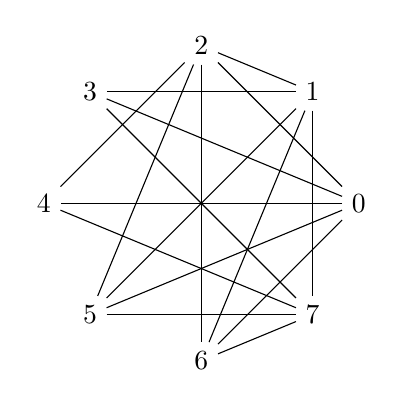
\begin{tikzpicture}
      \draw
        (0.0:2) node (0){0}
        (45.0:2) node (1){1}
        (90.0:2) node (2){2}
        (135.0:2) node (3){3}
        (180.0:2) node (4){4}
        (225.0:2) node (5){5}
        (270.0:2) node (6){6}
        (315.0:2) node (7){7};
      \begin{scope}[-]
        \draw (0) to (2);
        \draw (0) to (3);
        \draw (0) to (4);
        \draw (0) to (5);
        \draw (0) to (6);
        \draw (1) to (2);
        \draw (1) to (3);
        \draw (1) to (5);
        \draw (1) to (6);
        \draw (1) to (7);
        \draw (2) to (4);
        \draw (2) to (5);
        \draw (2) to (6);
        \draw (3) to (7);
        \draw (4) to (7);
        \draw (5) to (7);
        \draw (6) to (7);
      \end{scope}
    \end{tikzpicture}
\end{figure}
\begin{itemize}
\item signature: 0111110110111011100001001011
\item g: Graph with 8 nodes and 17 edges
\item order: 8
\item size: 17
\item max degree: 5
\item degrees: 3,3,4,4,5,5,5,5
\item is tree: 0
\item is bipartite: 0
\item has bridge: 0
\item is chordal: 0
\item is complete: 0
\item min cycle basis weight: 32
\item min cycle basis size: 10
\item diameter: 2
\item radius: 2
\item is eulerian: 0
\item is planar: 0
\item number of faces: 11
\item is regular: 0
\item p3: 34
\item p4: 10
\item property hash: 98de7409000b57f062c84380120914d07bcef5fb7b071c288fcc95dcb02f4e27
\end{itemize}
\newpage
\begin{figure}
  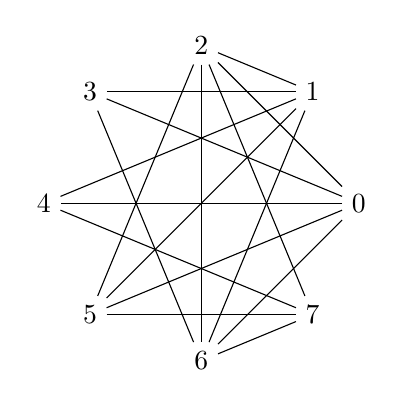
\begin{tikzpicture}
      \draw
        (0.0:2) node (0){0}
        (45.0:2) node (1){1}
        (90.0:2) node (2){2}
        (135.0:2) node (3){3}
        (180.0:2) node (4){4}
        (225.0:2) node (5){5}
        (270.0:2) node (6){6}
        (315.0:2) node (7){7};
      \begin{scope}[-]
        \draw (0) to (2);
        \draw (0) to (3);
        \draw (0) to (4);
        \draw (0) to (5);
        \draw (0) to (6);
        \draw (1) to (2);
        \draw (1) to (3);
        \draw (1) to (4);
        \draw (1) to (5);
        \draw (1) to (6);
        \draw (2) to (5);
        \draw (2) to (6);
        \draw (2) to (7);
        \draw (3) to (6);
        \draw (4) to (7);
        \draw (5) to (7);
        \draw (6) to (7);
      \end{scope}
    \end{tikzpicture}
\end{figure}
\begin{itemize}
\item signature: 0111110111110001110010001011
\item g: Graph with 8 nodes and 17 edges
\item order: 8
\item size: 17
\item max degree: 5
\item degrees: 3,3,4,4,5,5,5,5
\item is tree: 0
\item is bipartite: 0
\item has bridge: 0
\item is chordal: 0
\item is complete: 0
\item min cycle basis weight: 32
\item min cycle basis size: 10
\item diameter: 2
\item radius: 2
\item is eulerian: 0
\item is planar: 0
\item number of faces: 11
\item is regular: 0
\item p3: 34
\item p4: None
\item property hash: 2213b535dee08e2a0c942873752a590b2ca920292b9005099605fb5b7177c26b
\end{itemize}
\newpage
\begin{figure}
  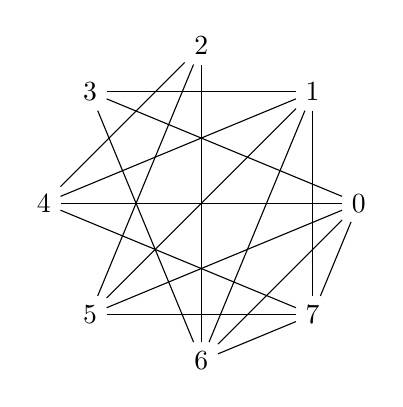
\begin{tikzpicture}
      \draw
        (0.0:2) node (0){0}
        (45.0:2) node (1){1}
        (90.0:2) node (2){2}
        (135.0:2) node (3){3}
        (180.0:2) node (4){4}
        (225.0:2) node (5){5}
        (270.0:2) node (6){6}
        (315.0:2) node (7){7};
      \begin{scope}[-]
        \draw (0) to (3);
        \draw (0) to (4);
        \draw (0) to (5);
        \draw (0) to (6);
        \draw (0) to (7);
        \draw (1) to (3);
        \draw (1) to (4);
        \draw (1) to (5);
        \draw (1) to (6);
        \draw (1) to (7);
        \draw (2) to (4);
        \draw (2) to (5);
        \draw (2) to (6);
        \draw (3) to (6);
        \draw (4) to (7);
        \draw (5) to (7);
        \draw (6) to (7);
      \end{scope}
    \end{tikzpicture}
\end{figure}
\begin{itemize}
\item signature: 0011111011111011100010001011
\item g: Graph with 8 nodes and 17 edges
\item order: 8
\item size: 17
\item max degree: 5
\item degrees: 3,3,4,4,5,5,5,5
\item is tree: 0
\item is bipartite: 0
\item has bridge: 0
\item is chordal: 0
\item is complete: 0
\item min cycle basis weight: 32
\item min cycle basis size: 10
\item diameter: 2
\item radius: 2
\item is eulerian: 0
\item is planar: 0
\item number of faces: 11
\item is regular: 0
\item p3: 34
\item p4: None
\item property hash: 2213b535dee08e2a0c942873752a590b2ca920292b9005099605fb5b7177c26b
\end{itemize}
\newpage
\begin{figure}
  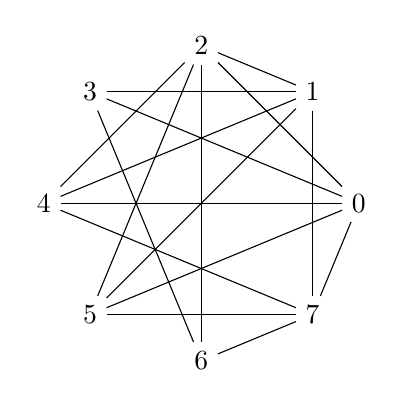
\begin{tikzpicture}
      \draw
        (0.0:2) node (0){0}
        (45.0:2) node (1){1}
        (90.0:2) node (2){2}
        (135.0:2) node (3){3}
        (180.0:2) node (4){4}
        (225.0:2) node (5){5}
        (270.0:2) node (6){6}
        (315.0:2) node (7){7};
      \begin{scope}[-]
        \draw (0) to (2);
        \draw (0) to (3);
        \draw (0) to (4);
        \draw (0) to (5);
        \draw (0) to (7);
        \draw (1) to (2);
        \draw (1) to (3);
        \draw (1) to (4);
        \draw (1) to (5);
        \draw (1) to (7);
        \draw (2) to (4);
        \draw (2) to (5);
        \draw (2) to (6);
        \draw (3) to (6);
        \draw (4) to (7);
        \draw (5) to (7);
        \draw (6) to (7);
      \end{scope}
    \end{tikzpicture}
\end{figure}
\begin{itemize}
\item signature: 0111101111101011100010001011
\item g: Graph with 8 nodes and 17 edges
\item order: 8
\item size: 17
\item max degree: 5
\item degrees: 3,3,4,4,5,5,5,5
\item is tree: 0
\item is bipartite: 0
\item has bridge: 0
\item is chordal: 0
\item is complete: 0
\item min cycle basis weight: 33
\item min cycle basis size: 10
\item diameter: 2
\item radius: 2
\item is eulerian: 0
\item is planar: 0
\item number of faces: 11
\item is regular: 0
\item p3: 34
\item p4: None
\item property hash: 1355db28c1bd818fe9c2b084bffce1ffb797ebecf0fb26d542a1672d084db9ab
\end{itemize}
\newpage
\begin{figure}
  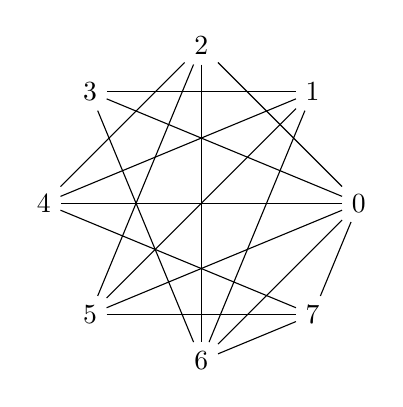
\begin{tikzpicture}
      \draw
        (0.0:2) node (0){0}
        (45.0:2) node (1){1}
        (90.0:2) node (2){2}
        (135.0:2) node (3){3}
        (180.0:2) node (4){4}
        (225.0:2) node (5){5}
        (270.0:2) node (6){6}
        (315.0:2) node (7){7};
      \begin{scope}[-]
        \draw (0) to (2);
        \draw (0) to (3);
        \draw (0) to (4);
        \draw (0) to (5);
        \draw (0) to (6);
        \draw (0) to (7);
        \draw (1) to (3);
        \draw (1) to (4);
        \draw (1) to (5);
        \draw (1) to (6);
        \draw (2) to (4);
        \draw (2) to (5);
        \draw (2) to (6);
        \draw (3) to (6);
        \draw (4) to (7);
        \draw (5) to (7);
        \draw (6) to (7);
      \end{scope}
    \end{tikzpicture}
\end{figure}
\begin{itemize}
\item signature: 0111111011110011100010001011
\item g: Graph with 8 nodes and 17 edges
\item order: 8
\item size: 17
\item max degree: 6
\item degrees: 3,4,4,4,4,4,5,6
\item is tree: 0
\item is bipartite: 0
\item has bridge: 0
\item is chordal: 0
\item is complete: 0
\item min cycle basis weight: 32
\item min cycle basis size: 10
\item diameter: 2
\item radius: 2
\item is eulerian: 0
\item is planar: 0
\item number of faces: 11
\item is regular: 0
\item p3: 34
\item p4: None
\item property hash: 112fd1a9939f0c6339f94a5a5455693cbb0b3a9acaa93a6532c6bad4a1466e03
\end{itemize}
\newpage
\begin{figure}
  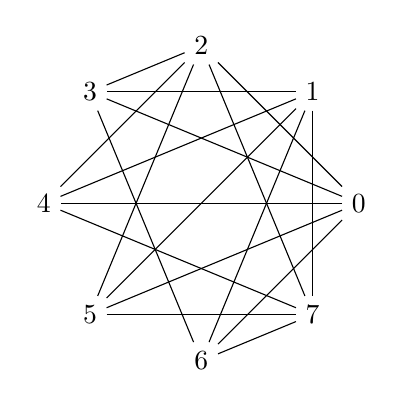
\begin{tikzpicture}
      \draw
        (0.0:2) node (0){0}
        (45.0:2) node (1){1}
        (90.0:2) node (2){2}
        (135.0:2) node (3){3}
        (180.0:2) node (4){4}
        (225.0:2) node (5){5}
        (270.0:2) node (6){6}
        (315.0:2) node (7){7};
      \begin{scope}[-]
        \draw (0) to (2);
        \draw (0) to (3);
        \draw (0) to (4);
        \draw (0) to (5);
        \draw (0) to (6);
        \draw (1) to (3);
        \draw (1) to (4);
        \draw (1) to (5);
        \draw (1) to (6);
        \draw (1) to (7);
        \draw (2) to (3);
        \draw (2) to (4);
        \draw (2) to (5);
        \draw (2) to (7);
        \draw (3) to (6);
        \draw (4) to (7);
        \draw (5) to (7);
        \draw (6) to (7);
      \end{scope}
    \end{tikzpicture}
\end{figure}
\begin{itemize}
\item signature: 0111110011111111010010001011
\item g: Graph with 8 nodes and 18 edges
\item order: 8
\item size: 18
\item max degree: 5
\item degrees: 4,4,4,4,5,5,5,5
\item is tree: 0
\item is bipartite: 0
\item has bridge: 0
\item is chordal: 0
\item is complete: 0
\item min cycle basis weight: 34
\item min cycle basis size: 11
\item diameter: 2
\item radius: 2
\item is eulerian: 0
\item is planar: 0
\item number of faces: 12
\item is regular: 0
\item p3: 34
\item p4: 11
\item property hash: e4f90969050dc86106ad1d3faf86b149dc483afd060ccf149dda051244f167b0
\end{itemize}
\newpage
\begin{figure}
  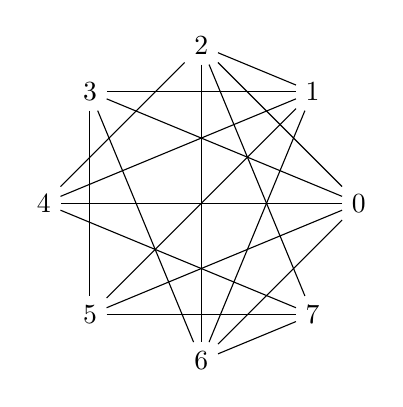
\begin{tikzpicture}
      \draw
        (0.0:2) node (0){0}
        (45.0:2) node (1){1}
        (90.0:2) node (2){2}
        (135.0:2) node (3){3}
        (180.0:2) node (4){4}
        (225.0:2) node (5){5}
        (270.0:2) node (6){6}
        (315.0:2) node (7){7};
      \begin{scope}[-]
        \draw (0) to (2);
        \draw (0) to (3);
        \draw (0) to (4);
        \draw (0) to (5);
        \draw (0) to (6);
        \draw (1) to (2);
        \draw (1) to (3);
        \draw (1) to (4);
        \draw (1) to (5);
        \draw (1) to (6);
        \draw (2) to (4);
        \draw (2) to (6);
        \draw (2) to (7);
        \draw (3) to (5);
        \draw (3) to (6);
        \draw (4) to (7);
        \draw (5) to (7);
        \draw (6) to (7);
      \end{scope}
    \end{tikzpicture}
\end{figure}
\begin{itemize}
\item signature: 0111110111110010110110001011
\item g: Graph with 8 nodes and 18 edges
\item order: 8
\item size: 18
\item max degree: 5
\item degrees: 4,4,4,4,5,5,5,5
\item is tree: 0
\item is bipartite: 0
\item has bridge: 0
\item is chordal: 0
\item is complete: 0
\item min cycle basis weight: 34
\item min cycle basis size: 11
\item diameter: 2
\item radius: 2
\item is eulerian: 0
\item is planar: 0
\item number of faces: 12
\item is regular: 0
\item p3: 34
\item p4: None
\item property hash: e1ad2b825937448c612038ca32fdb59d40d5ccd66975a536273d430692db9250
\end{itemize}
\newpage
\begin{figure}
  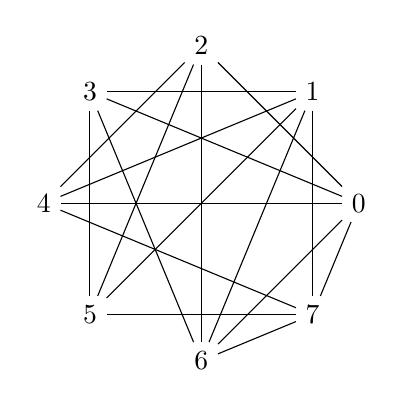
\begin{tikzpicture}
      \draw
        (0.0:2) node (0){0}
        (45.0:2) node (1){1}
        (90.0:2) node (2){2}
        (135.0:2) node (3){3}
        (180.0:2) node (4){4}
        (225.0:2) node (5){5}
        (270.0:2) node (6){6}
        (315.0:2) node (7){7};
      \begin{scope}[-]
        \draw (0) to (2);
        \draw (0) to (3);
        \draw (0) to (4);
        \draw (0) to (6);
        \draw (0) to (7);
        \draw (1) to (3);
        \draw (1) to (4);
        \draw (1) to (5);
        \draw (1) to (6);
        \draw (1) to (7);
        \draw (2) to (4);
        \draw (2) to (5);
        \draw (2) to (6);
        \draw (3) to (5);
        \draw (3) to (6);
        \draw (4) to (7);
        \draw (5) to (7);
        \draw (6) to (7);
      \end{scope}
    \end{tikzpicture}
\end{figure}
\begin{itemize}
\item signature: 0111011011111011100110001011
\item g: Graph with 8 nodes and 18 edges
\item order: 8
\item size: 18
\item max degree: 5
\item degrees: 4,4,4,4,5,5,5,5
\item is tree: 0
\item is bipartite: 0
\item has bridge: 0
\item is chordal: 0
\item is complete: 0
\item min cycle basis weight: 34
\item min cycle basis size: 11
\item diameter: 2
\item radius: 2
\item is eulerian: 0
\item is planar: 0
\item number of faces: 12
\item is regular: 0
\item p3: 34
\item p4: 11
\item property hash: e4f90969050dc86106ad1d3faf86b149dc483afd060ccf149dda051244f167b0
\end{itemize}
\newpage
\begin{figure}
  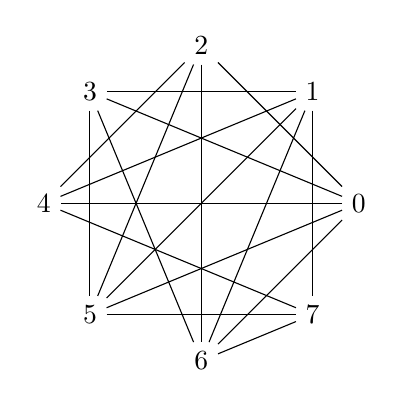
\begin{tikzpicture}
      \draw
        (0.0:2) node (0){0}
        (45.0:2) node (1){1}
        (90.0:2) node (2){2}
        (135.0:2) node (3){3}
        (180.0:2) node (4){4}
        (225.0:2) node (5){5}
        (270.0:2) node (6){6}
        (315.0:2) node (7){7};
      \begin{scope}[-]
        \draw (0) to (2);
        \draw (0) to (3);
        \draw (0) to (4);
        \draw (0) to (5);
        \draw (0) to (6);
        \draw (1) to (3);
        \draw (1) to (4);
        \draw (1) to (5);
        \draw (1) to (6);
        \draw (1) to (7);
        \draw (2) to (4);
        \draw (2) to (5);
        \draw (2) to (6);
        \draw (3) to (5);
        \draw (3) to (6);
        \draw (4) to (7);
        \draw (5) to (7);
        \draw (6) to (7);
      \end{scope}
    \end{tikzpicture}
\end{figure}
\begin{itemize}
\item signature: 0111110011111011100110001011
\item g: Graph with 8 nodes and 18 edges
\item order: 8
\item size: 18
\item max degree: 5
\item degrees: 4,4,4,4,5,5,5,5
\item is tree: 0
\item is bipartite: 0
\item has bridge: 0
\item is chordal: 0
\item is complete: 0
\item min cycle basis weight: 34
\item min cycle basis size: 11
\item diameter: 2
\item radius: 2
\item is eulerian: 0
\item is planar: 0
\item number of faces: 12
\item is regular: 0
\item p3: 34
\item p4: None
\item property hash: e1ad2b825937448c612038ca32fdb59d40d5ccd66975a536273d430692db9250
\end{itemize}
\newpage
\begin{figure}
  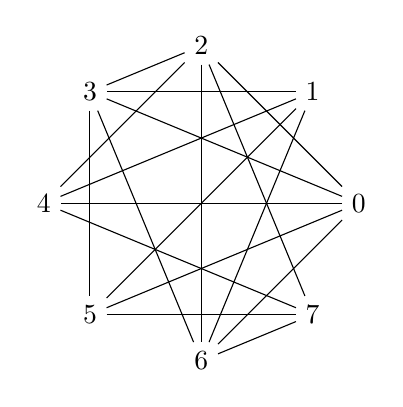
\begin{tikzpicture}
      \draw
        (0.0:2) node (0){0}
        (45.0:2) node (1){1}
        (90.0:2) node (2){2}
        (135.0:2) node (3){3}
        (180.0:2) node (4){4}
        (225.0:2) node (5){5}
        (270.0:2) node (6){6}
        (315.0:2) node (7){7};
      \begin{scope}[-]
        \draw (0) to (2);
        \draw (0) to (3);
        \draw (0) to (4);
        \draw (0) to (5);
        \draw (0) to (6);
        \draw (1) to (3);
        \draw (1) to (4);
        \draw (1) to (5);
        \draw (1) to (6);
        \draw (2) to (3);
        \draw (2) to (4);
        \draw (2) to (6);
        \draw (2) to (7);
        \draw (3) to (5);
        \draw (3) to (6);
        \draw (4) to (7);
        \draw (5) to (7);
        \draw (6) to (7);
      \end{scope}
    \end{tikzpicture}
\end{figure}
\begin{itemize}
\item signature: 0111110011110110110110001011
\item g: Graph with 8 nodes and 18 edges
\item order: 8
\item size: 18
\item max degree: 5
\item degrees: 4,4,4,4,5,5,5,5
\item is tree: 0
\item is bipartite: 0
\item has bridge: 0
\item is chordal: 0
\item is complete: 0
\item min cycle basis weight: 35
\item min cycle basis size: 11
\item diameter: 2
\item radius: 2
\item is eulerian: 0
\item is planar: 0
\item number of faces: 12
\item is regular: 0
\item p3: 34
\item p4: None
\item property hash: 91e6f0adbee2f84762f8b3bf41309effa70890de403074030479bdf8e98aa0c3
\end{itemize}
\newpage
\begin{figure}
  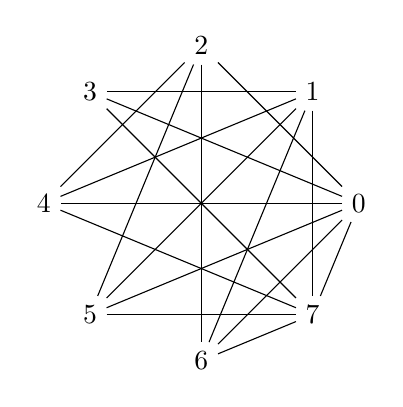
\begin{tikzpicture}
      \draw
        (0.0:2) node (0){0}
        (45.0:2) node (1){1}
        (90.0:2) node (2){2}
        (135.0:2) node (3){3}
        (180.0:2) node (4){4}
        (225.0:2) node (5){5}
        (270.0:2) node (6){6}
        (315.0:2) node (7){7};
      \begin{scope}[-]
        \draw (0) to (2);
        \draw (0) to (3);
        \draw (0) to (4);
        \draw (0) to (5);
        \draw (0) to (6);
        \draw (0) to (7);
        \draw (1) to (3);
        \draw (1) to (4);
        \draw (1) to (5);
        \draw (1) to (6);
        \draw (1) to (7);
        \draw (2) to (4);
        \draw (2) to (5);
        \draw (2) to (6);
        \draw (3) to (7);
        \draw (4) to (7);
        \draw (5) to (7);
        \draw (6) to (7);
      \end{scope}
    \end{tikzpicture}
\end{figure}
\begin{itemize}
\item signature: 0111111011111011100001001011
\item g: Graph with 8 nodes and 18 edges
\item order: 8
\item size: 18
\item max degree: 6
\item degrees: 3,4,4,4,4,5,6,6
\item is tree: 0
\item is bipartite: 0
\item has bridge: 0
\item is chordal: 0
\item is complete: 0
\item min cycle basis weight: 33
\item min cycle basis size: 11
\item diameter: 2
\item radius: 2
\item is eulerian: 0
\item is planar: 0
\item number of faces: 12
\item is regular: 0
\item p3: 34
\item p4: None
\item property hash: 6cfd326f5130e3edb7ab0f3b57ee17f21ae9f92a0ee104508c513016f6fba4c7
\end{itemize}
\newpage
\begin{figure}
  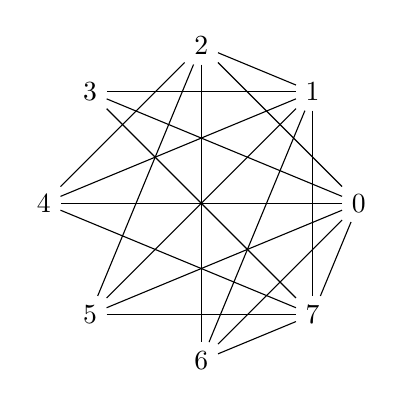
\begin{tikzpicture}
      \draw
        (0.0:2) node (0){0}
        (45.0:2) node (1){1}
        (90.0:2) node (2){2}
        (135.0:2) node (3){3}
        (180.0:2) node (4){4}
        (225.0:2) node (5){5}
        (270.0:2) node (6){6}
        (315.0:2) node (7){7};
      \begin{scope}[-]
        \draw (0) to (2);
        \draw (0) to (3);
        \draw (0) to (4);
        \draw (0) to (5);
        \draw (0) to (6);
        \draw (0) to (7);
        \draw (1) to (2);
        \draw (1) to (3);
        \draw (1) to (4);
        \draw (1) to (5);
        \draw (1) to (6);
        \draw (1) to (7);
        \draw (2) to (4);
        \draw (2) to (5);
        \draw (2) to (6);
        \draw (3) to (7);
        \draw (4) to (7);
        \draw (5) to (7);
        \draw (6) to (7);
      \end{scope}
    \end{tikzpicture}
\end{figure}
\begin{itemize}
\item signature: 0111111111111011100001001011
\item g: Graph with 8 nodes and 19 edges
\item order: 8
\item size: 19
\item max degree: 6
\item degrees: 3,4,4,4,5,6,6,6
\item is tree: 0
\item is bipartite: 0
\item has bridge: 0
\item is chordal: 0
\item is complete: 0
\item min cycle basis weight: 36
\item min cycle basis size: 12
\item diameter: 2
\item radius: 2
\item is eulerian: 0
\item is planar: 0
\item number of faces: 13
\item is regular: 0
\item p3: 34
\item p4: None
\item property hash: 01de12546d057783001778658e22cde1d10c74dc82696c0e6802bf36273f69fb
\end{itemize}
\newpage
\begin{figure}
  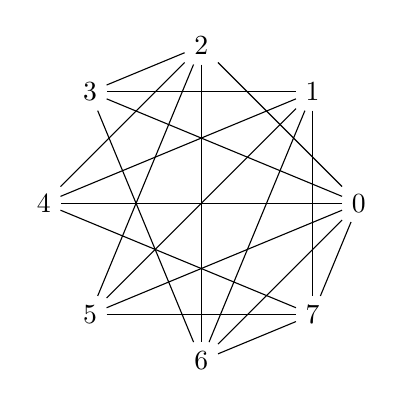
\begin{tikzpicture}
      \draw
        (0.0:2) node (0){0}
        (45.0:2) node (1){1}
        (90.0:2) node (2){2}
        (135.0:2) node (3){3}
        (180.0:2) node (4){4}
        (225.0:2) node (5){5}
        (270.0:2) node (6){6}
        (315.0:2) node (7){7};
      \begin{scope}[-]
        \draw (0) to (2);
        \draw (0) to (3);
        \draw (0) to (4);
        \draw (0) to (5);
        \draw (0) to (6);
        \draw (0) to (7);
        \draw (1) to (3);
        \draw (1) to (4);
        \draw (1) to (5);
        \draw (1) to (6);
        \draw (1) to (7);
        \draw (2) to (3);
        \draw (2) to (4);
        \draw (2) to (5);
        \draw (2) to (6);
        \draw (3) to (6);
        \draw (4) to (7);
        \draw (5) to (7);
        \draw (6) to (7);
      \end{scope}
    \end{tikzpicture}
\end{figure}
\begin{itemize}
\item signature: 0111111011111111100010001011
\item g: Graph with 8 nodes and 19 edges
\item order: 8
\item size: 19
\item max degree: 6
\item degrees: 4,4,4,5,5,5,5,6
\item is tree: 0
\item is bipartite: 0
\item has bridge: 0
\item is chordal: 0
\item is complete: 0
\item min cycle basis weight: 36
\item min cycle basis size: 12
\item diameter: 2
\item radius: 2
\item is eulerian: 0
\item is planar: 0
\item number of faces: 13
\item is regular: 0
\item p3: 34
\item p4: None
\item property hash: 745ab0532a93cbdd3de0561b50029bf25c88964859af4290f1986380f04f7c1a
\end{itemize}
\newpage
\begin{figure}
  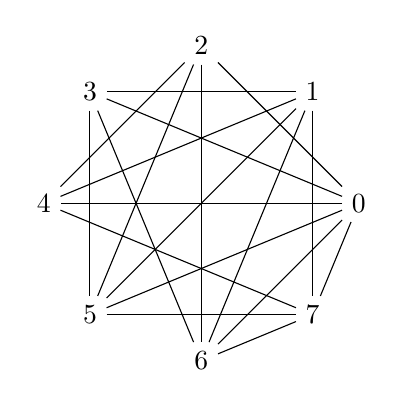
\begin{tikzpicture}
      \draw
        (0.0:2) node (0){0}
        (45.0:2) node (1){1}
        (90.0:2) node (2){2}
        (135.0:2) node (3){3}
        (180.0:2) node (4){4}
        (225.0:2) node (5){5}
        (270.0:2) node (6){6}
        (315.0:2) node (7){7};
      \begin{scope}[-]
        \draw (0) to (2);
        \draw (0) to (3);
        \draw (0) to (4);
        \draw (0) to (5);
        \draw (0) to (6);
        \draw (0) to (7);
        \draw (1) to (3);
        \draw (1) to (4);
        \draw (1) to (5);
        \draw (1) to (6);
        \draw (1) to (7);
        \draw (2) to (4);
        \draw (2) to (5);
        \draw (2) to (6);
        \draw (3) to (5);
        \draw (3) to (6);
        \draw (4) to (7);
        \draw (5) to (7);
        \draw (6) to (7);
      \end{scope}
    \end{tikzpicture}
\end{figure}
\begin{itemize}
\item signature: 0111111011111011100110001011
\item g: Graph with 8 nodes and 19 edges
\item order: 8
\item size: 19
\item max degree: 6
\item degrees: 4,4,4,5,5,5,5,6
\item is tree: 0
\item is bipartite: 0
\item has bridge: 0
\item is chordal: 0
\item is complete: 0
\item min cycle basis weight: 36
\item min cycle basis size: 12
\item diameter: 2
\item radius: 2
\item is eulerian: 0
\item is planar: 0
\item number of faces: 13
\item is regular: 0
\item p3: 34
\item p4: None
\item property hash: 745ab0532a93cbdd3de0561b50029bf25c88964859af4290f1986380f04f7c1a
\end{itemize}
\newpage
\begin{figure}
  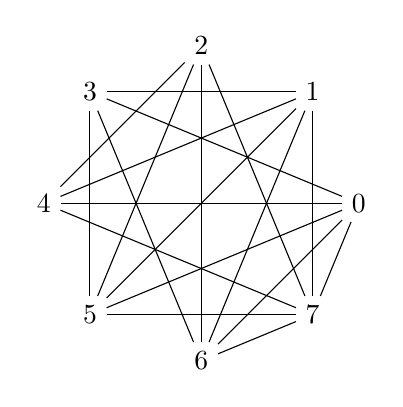
\begin{tikzpicture}
      \draw
        (0.0:2) node (0){0}
        (45.0:2) node (1){1}
        (90.0:2) node (2){2}
        (135.0:2) node (3){3}
        (180.0:2) node (4){4}
        (225.0:2) node (5){5}
        (270.0:2) node (6){6}
        (315.0:2) node (7){7};
      \begin{scope}[-]
        \draw (0) to (3);
        \draw (0) to (4);
        \draw (0) to (5);
        \draw (0) to (6);
        \draw (0) to (7);
        \draw (1) to (3);
        \draw (1) to (4);
        \draw (1) to (5);
        \draw (1) to (6);
        \draw (1) to (7);
        \draw (2) to (4);
        \draw (2) to (5);
        \draw (2) to (6);
        \draw (2) to (7);
        \draw (3) to (5);
        \draw (3) to (6);
        \draw (4) to (7);
        \draw (5) to (7);
        \draw (6) to (7);
      \end{scope}
    \end{tikzpicture}
\end{figure}
\begin{itemize}
\item signature: 0011111011111011110110001011
\item g: Graph with 8 nodes and 19 edges
\item order: 8
\item size: 19
\item max degree: 6
\item degrees: 4,4,4,5,5,5,5,6
\item is tree: 0
\item is bipartite: 0
\item has bridge: 0
\item is chordal: 0
\item is complete: 0
\item min cycle basis weight: 36
\item min cycle basis size: 12
\item diameter: 2
\item radius: 2
\item is eulerian: 0
\item is planar: 0
\item number of faces: 13
\item is regular: 0
\item p3: 34
\item p4: None
\item property hash: 745ab0532a93cbdd3de0561b50029bf25c88964859af4290f1986380f04f7c1a
\end{itemize}
\newpage
\begin{figure}
  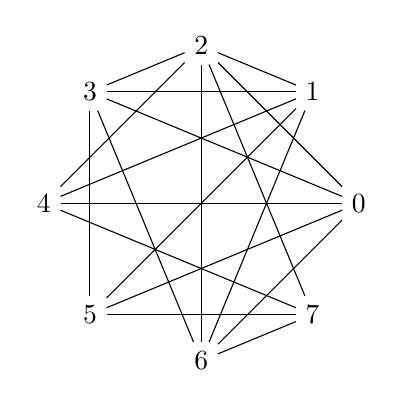
\begin{tikzpicture}
      \draw
        (0.0:2) node (0){0}
        (45.0:2) node (1){1}
        (90.0:2) node (2){2}
        (135.0:2) node (3){3}
        (180.0:2) node (4){4}
        (225.0:2) node (5){5}
        (270.0:2) node (6){6}
        (315.0:2) node (7){7};
      \begin{scope}[-]
        \draw (0) to (2);
        \draw (0) to (3);
        \draw (0) to (4);
        \draw (0) to (5);
        \draw (0) to (6);
        \draw (1) to (2);
        \draw (1) to (3);
        \draw (1) to (4);
        \draw (1) to (5);
        \draw (1) to (6);
        \draw (2) to (3);
        \draw (2) to (4);
        \draw (2) to (6);
        \draw (2) to (7);
        \draw (3) to (5);
        \draw (3) to (6);
        \draw (4) to (7);
        \draw (5) to (7);
        \draw (6) to (7);
      \end{scope}
    \end{tikzpicture}
\end{figure}
\begin{itemize}
\item signature: 0111110111110110110110001011
\item g: Graph with 8 nodes and 19 edges
\item order: 8
\item size: 19
\item max degree: 6
\item degrees: 4,4,4,5,5,5,5,6
\item is tree: 0
\item is bipartite: 0
\item has bridge: 0
\item is chordal: 0
\item is complete: 0
\item min cycle basis weight: 37
\item min cycle basis size: 12
\item diameter: 2
\item radius: 2
\item is eulerian: 0
\item is planar: 0
\item number of faces: 13
\item is regular: 0
\item p3: 34
\item p4: None
\item property hash: 0c717213a5193eb6b31400b117c9fd94d5f9a4066e8234f19395b72caec1c669
\end{itemize}
\newpage
\begin{figure}
  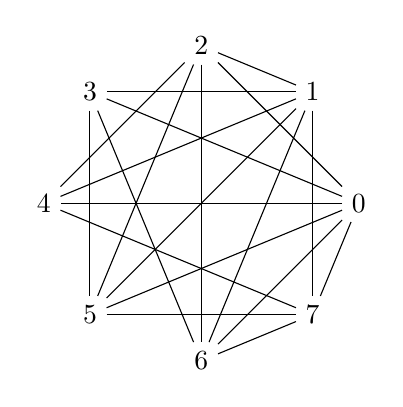
\begin{tikzpicture}
      \draw
        (0.0:2) node (0){0}
        (45.0:2) node (1){1}
        (90.0:2) node (2){2}
        (135.0:2) node (3){3}
        (180.0:2) node (4){4}
        (225.0:2) node (5){5}
        (270.0:2) node (6){6}
        (315.0:2) node (7){7};
      \begin{scope}[-]
        \draw (0) to (2);
        \draw (0) to (3);
        \draw (0) to (4);
        \draw (0) to (5);
        \draw (0) to (6);
        \draw (0) to (7);
        \draw (1) to (2);
        \draw (1) to (3);
        \draw (1) to (4);
        \draw (1) to (5);
        \draw (1) to (6);
        \draw (1) to (7);
        \draw (2) to (4);
        \draw (2) to (5);
        \draw (2) to (6);
        \draw (3) to (5);
        \draw (3) to (6);
        \draw (4) to (7);
        \draw (5) to (7);
        \draw (6) to (7);
      \end{scope}
    \end{tikzpicture}
\end{figure}
\begin{itemize}
\item signature: 0111111111111011100110001011
\item g: Graph with 8 nodes and 20 edges
\item order: 8
\item size: 20
\item max degree: 6
\item degrees: 4,4,5,5,5,5,6,6
\item is tree: 0
\item is bipartite: 0
\item has bridge: 0
\item is chordal: 0
\item is complete: 0
\item min cycle basis weight: 39
\item min cycle basis size: 13
\item diameter: 2
\item radius: 2
\item is eulerian: 0
\item is planar: 0
\item number of faces: 14
\item is regular: 0
\item p3: 34
\item p4: None
\item property hash: 070733cc8f8921a92debe4807c4f12e6326420dbd2dd2d0fcc7b7ad475ce1b8c
\end{itemize}
\newpage
\begin{figure}
  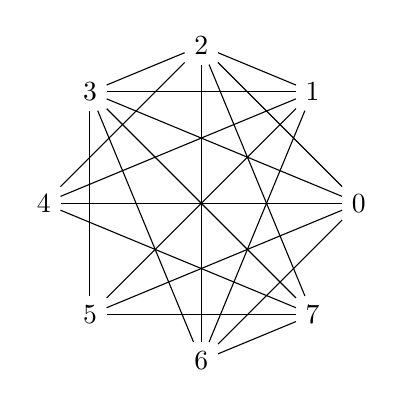
\begin{tikzpicture}
      \draw
        (0.0:2) node (0){0}
        (45.0:2) node (1){1}
        (90.0:2) node (2){2}
        (135.0:2) node (3){3}
        (180.0:2) node (4){4}
        (225.0:2) node (5){5}
        (270.0:2) node (6){6}
        (315.0:2) node (7){7};
      \begin{scope}[-]
        \draw (0) to (2);
        \draw (0) to (3);
        \draw (0) to (4);
        \draw (0) to (5);
        \draw (0) to (6);
        \draw (1) to (2);
        \draw (1) to (3);
        \draw (1) to (4);
        \draw (1) to (5);
        \draw (1) to (6);
        \draw (2) to (3);
        \draw (2) to (4);
        \draw (2) to (6);
        \draw (2) to (7);
        \draw (3) to (5);
        \draw (3) to (6);
        \draw (3) to (7);
        \draw (4) to (7);
        \draw (5) to (7);
        \draw (6) to (7);
      \end{scope}
    \end{tikzpicture}
\end{figure}
\begin{itemize}
\item signature: 0111110111110110110111001011
\item g: Graph with 8 nodes and 20 edges
\item order: 8
\item size: 20
\item max degree: 6
\item degrees: 4,4,5,5,5,5,6,6
\item is tree: 0
\item is bipartite: 0
\item has bridge: 0
\item is chordal: 0
\item is complete: 0
\item min cycle basis weight: 39
\item min cycle basis size: 13
\item diameter: 2
\item radius: 2
\item is eulerian: 0
\item is planar: 0
\item number of faces: 14
\item is regular: 0
\item p3: 34
\item p4: None
\item property hash: 070733cc8f8921a92debe4807c4f12e6326420dbd2dd2d0fcc7b7ad475ce1b8c
\end{itemize}
\newpage
\begin{figure}
  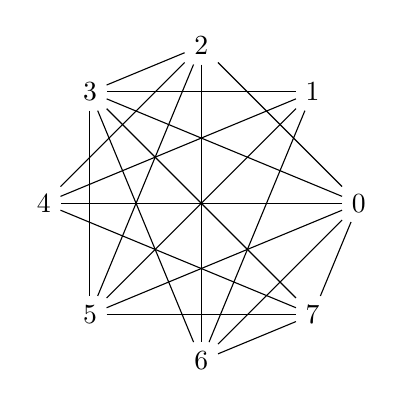
\begin{tikzpicture}
      \draw
        (0.0:2) node (0){0}
        (45.0:2) node (1){1}
        (90.0:2) node (2){2}
        (135.0:2) node (3){3}
        (180.0:2) node (4){4}
        (225.0:2) node (5){5}
        (270.0:2) node (6){6}
        (315.0:2) node (7){7};
      \begin{scope}[-]
        \draw (0) to (2);
        \draw (0) to (3);
        \draw (0) to (4);
        \draw (0) to (5);
        \draw (0) to (6);
        \draw (0) to (7);
        \draw (1) to (3);
        \draw (1) to (4);
        \draw (1) to (5);
        \draw (1) to (6);
        \draw (2) to (3);
        \draw (2) to (4);
        \draw (2) to (5);
        \draw (2) to (6);
        \draw (3) to (5);
        \draw (3) to (6);
        \draw (3) to (7);
        \draw (4) to (7);
        \draw (5) to (7);
        \draw (6) to (7);
      \end{scope}
    \end{tikzpicture}
\end{figure}
\begin{itemize}
\item signature: 0111111011110111100111001011
\item g: Graph with 8 nodes and 20 edges
\item order: 8
\item size: 20
\item max degree: 6
\item degrees: 4,4,5,5,5,5,6,6
\item is tree: 0
\item is bipartite: 0
\item has bridge: 0
\item is chordal: 0
\item is complete: 0
\item min cycle basis weight: 40
\item min cycle basis size: 13
\item diameter: 2
\item radius: 2
\item is eulerian: 0
\item is planar: 0
\item number of faces: 14
\item is regular: 0
\item p3: 34
\item p4: None
\item property hash: 9a8f253a19dcd778f0fe679e270009ed998d1f3fa3612bfe504ee0003f4b807c
\end{itemize}
\newpage
